\documentclass[aspectratio=169,usenames,dvipsnames]{beamer}

\usepackage{amsmath}
\usepackage{booktabs}
\usepackage{xcolor}
\usepackage[english]{babel}
\usepackage{unicode-math}
\usepackage{mathtools}
\usepackage{derivative}
\usepackage{makecell}
\usepackage{multirow}
\usepackage{siunitx}
\usepackage{pgfplots}
\usepackage{appendixnumberbeamer}

\usetheme{metropolis}

\setmainfont{Stix Two Text}
\setmathfont{Stix Two Math}

\DeclarePairedDelimiter{\ceil}{\lceil}{\rceil}
\DeclarePairedDelimiter{\floor}{\lfloor}{\rfloor}
\DeclarePairedDelimiter{\abs}{\lvert}{\rvert}
\DeclarePairedDelimiter{\norm}{\lVert}{\rVert}
\DeclarePairedDelimiter{\bra}{\langle}{\rvert}
\DeclarePairedDelimiter{\ket}{\lvert}{\rangle}
\DeclarePairedDelimiter{\expval}{\langle}{\rangle}
\DeclarePairedDelimiter{\norder}{\mathcolon}{\mathcolon}
\DeclarePairedDelimiter{\anorder}{\typecolon}{\typecolon}
	
\newcommand{\laplace}{\mbfnabla^2}
\newcommand{\trans}{{\scriptscriptstyle\mathsf{T}}}

\newcommand{\conv}{\ast}
\newcommand{\vdot}{\cdot}
\newcommand{\vcross}{\vectimes}
\newcommand{\vb}[1]{\symbfup{#1}}
\newcommand{\vu}[1]{\hat{\vb{#1}}}
\newcommand*\dd[2][\relax]{\mathop{\ifx\relax#1\odif{#2}\else \odif[order={#1}]{#2}\fi}}

\newcommand{\vacket}{\ket*{0}}
\newcommand{\vacbra}{\bra*{0}}

\DeclareMathOperator{\trace}{Tr}
\DeclareMathOperator{\sinc}{sinc}

\AtBeginDocument{
	\let\Re\relax
	\let\Im\relax
	\DeclareMathOperator{\Re}{Re}
	\DeclareMathOperator{\Im}{Im}

	\renewcommand{\div}{\mathop{\mbfnabla\vdot}}
	\newcommand{\curl}{\mathop{\mbfnabla\vectimes}}
}

\DeclarePairedDelimiterX{\comm}[2]{[}{]}{#1,#2}

\DeclarePairedDelimiterX{\braket}[2]{\langle}{\rangle}{#1\delimsize\vert#2}
\DeclarePairedDelimiterX{\ketbra}[1]{\lvert}{\rvert}{#1\rangle\delimsize\langle#1}


\usetikzlibrary{arrows.meta,fit,mindmap,positioning}

\definecolor{exotic orange}{RGB}{255,128,0}
\definecolor{exotic green}{RGB}{0,102,102}
\definecolor{exotic blue}{RGB}{67,132,161}
\definecolor{exotic red}{RGB}{250,86,86}

\title{A theoretical framework for CV-QKD}
\date{\today}
\author{Bodo Kaiser}
\institute{Ludwig-Maximilians-Universität München}

\begin{document}
	\maketitle
	
	\begin{frame}
		\begin{center}
			\textbf{Prelude}
			
			What is light?
		\end{center}
	\end{frame}
	
	% why is QKD interesting? -> intersection of multiple disciplines (quantum information theory, quantum optics, communication engineering)	
	\begin{frame}{Preview}
		\begin{columns}[c, onlytextwidth]
			\column{0.5\textwidth}
			\setbeamertemplate{section in toc}[sections numbered]
			\tableofcontents[hideallsubsections]
			
			\column{0.5\textwidth}
			\begin{figure}
				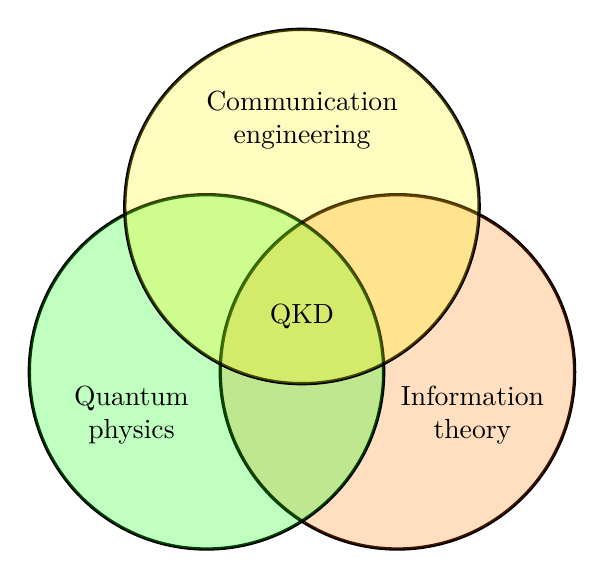
\begin{tikzpicture}[
					venn circle/.style={draw, very thick, fill opacity=0.25, circle, minimum width=45mm},
					venn label/.style={align=center},
				]
					\begin{scope}[blend group=soft light]
						\node[venn circle, fill=yellow] (qp) at (90:1.4) {};
						\node[venn circle, fill=green] (it) at (210:1.4) {};
						\node[venn circle, fill=orange] (qp) at (330:1.4) {};
					\end{scope}
					
					\node[venn label] {QKD};
					\node[venn label] at (90:2.5) {Communication\\engineering};
					\node[venn label] at (210:2.5) {Quantum\\physics};
					\node[venn label] at (330:2.5) {Information\\theory};
				\end{tikzpicture}
			\end{figure}
		\end{columns}
	\end{frame}
	
	\section{Quantum key distribution}

	% what is secure communication: integrity and confidentiality	
	% key distribution problem
	% public-key distribution
	% information-theoretical secure for OTP but practically one uses AES
	\begin{frame}{Secure communication}
		\begin{figure}
			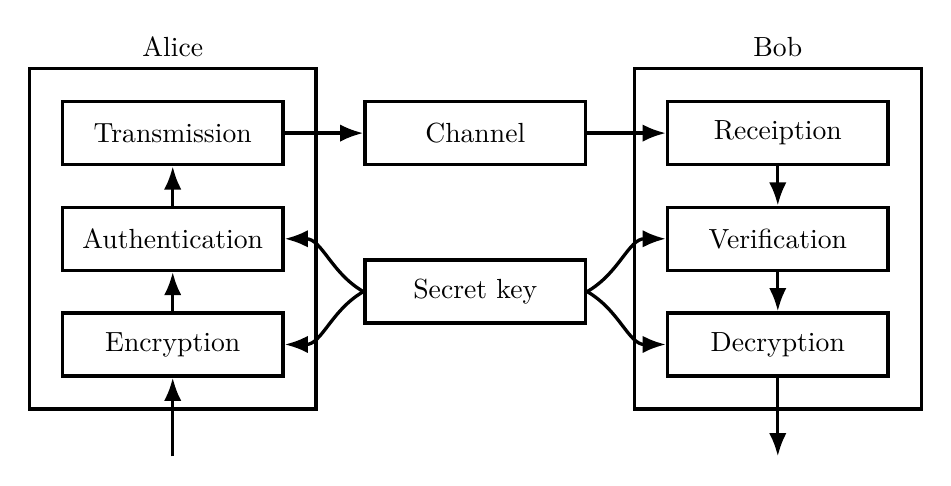
\begin{tikzpicture}[
				node distance=5mm,
				arrow/.style={very thick, -Latex},
				block/.style={draw, very thick, minimum width=28mm, minimum height=8mm},		
				superblock/.style={draw, very thick, inner sep=4mm},
			]
				\coordinate (in);
				\node[block, above=10mm of in] (encryption) {Encryption};
				\node[block, above=of encryption] (authentication) {Authentication};
				\node[block, above=of authentication] (transmitter) {Transmission};
				\node[block, right=10mm of transmitter] (channel) {Channel};
				\node[block, right=10mm of channel] (receiver) {Receiption};
				\node[block, below=of receiver] (verification) {Verification};
				\node[block, below=of verification] (decryption) {Decryption};
				\coordinate[below=10mm of decryption] (out);
	
				\path (encryption) -- (verification) node[midway, block] (key) {Secret key};
	
				\draw[arrow] (key.west) to[out=210, in=0] (encryption.east);
				\draw[arrow] (key.west) to[out=150, in=0]  (authentication.east);
				\draw[arrow] (key.east) to[out=-30, in=180] (decryption.west);
				\draw[arrow] (key.east) to[out=30, in=180] (verification.west);

				\draw[arrow] (in) -- (encryption);
				\draw[arrow] (encryption) -- (authentication);
				\draw[arrow] (authentication) -- (transmitter);
				
				\draw[arrow] (decryption) -- (out);
				\draw[arrow] (verification) -- (decryption);
				\draw[arrow] (receiver) -- (verification);
		
				\draw[arrow] (transmitter) -- (channel.west);
				\draw[arrow] (channel.east) -- (receiver);
				
				\node[superblock, label={Alice}, fit=(encryption) (transmitter)] {};
				\node[superblock, label={Bob}, fit=(decryption) (receiver)] {};
			\end{tikzpicture}
			\caption{Block diagram of a secure transmission system.}
		\end{figure}
	\end{frame}

    % quantum transmission (random seed, correlated data)
	% post-processing (shared secret key from correlated data)
	\begin{frame}{Quantum key distribution}
		\begin{figure}
			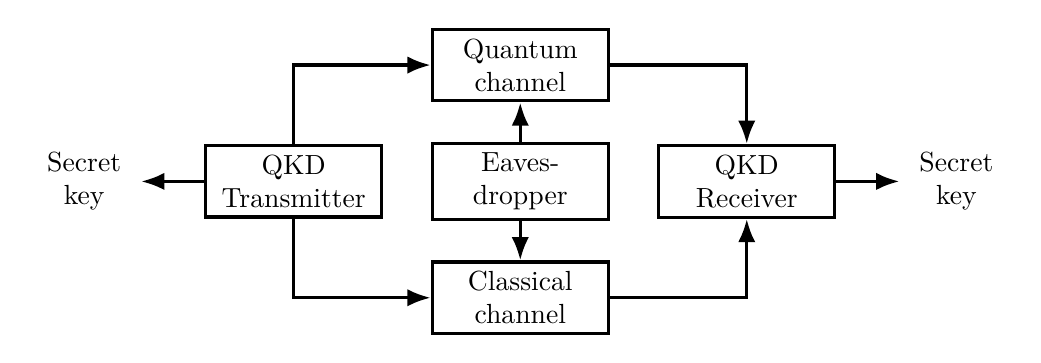
\begin{tikzpicture}[
				node distance=5mm,
				arrow/.style={very thick, -Latex},
				block/.style={draw, very thick, minimum width=20mm, minimum height=8mm, text width=20mm, align=center},
				superblock/.style={draw, very thick, inner sep=3mm},
			]
				\node[block] (transmitter) {QKD Transmitter};
				\node[text width=12mm, align=center, left=8mm of transmitter] (alice key) {Secret key};
	
				\node[block, right=6mm of transmitter] (eve) {Eavesdropper};
				\node[block, above=5mm of eve] (quantum channel) {Quantum channel};
				\node[block, below=5mm of eve] (classical channel) {Classical channel};
				\node[block, right=6mm of eve] (receiver) {QKD Receiver};
				\node[text width=12mm, align=center, right=8mm of receiver] (bob key) {Secret key};
				
				\draw[arrow] (transmitter) -- (alice key);
				\draw[arrow] (receiver) -- (bob key);
				\draw[arrow] (eve) -- (classical channel);
				\draw[arrow] (eve) -- (quantum channel);
				\draw[arrow] (transmitter.north) -- (transmitter.north|-quantum channel.west) -- (quantum channel.west);
				\draw[arrow] (transmitter.south) -- (transmitter.south|-classical channel.west) -- (classical channel.west);
				\draw[arrow] (quantum channel.east) -- (quantum channel.east-|receiver.north) -- (receiver.north);
				\draw[arrow] (classical channel.east) -- (classical channel.east-|receiver.south) -- (receiver.south);
				
				%\node[superblock, label={Alice}, fit=(alice key) (transmitter)] {};
				%\node[superblock, label={Bob}, fit=(bob key) (receiver)] {};
			\end{tikzpicture}
			\caption{Block diagram of a QKD system.}
		\end{figure}
	\end{frame}
	
	\begin{frame}{Taxonomy of QKD protocols}
		\begin{table}
			\caption{Summary of common characteristics among QKD protocols.}
			\begin{tabular}{lc}
				\toprule
				& Typical chacteristics \\
				\midrule
				Schema & Entanglement-based or prepare-and-measure \\
				Detection & Coherent or single-photon \\
				\makecell[l]{Measurement-\\basis selection} & Active or passive \\
				Logical encoding & Qubit or Boson \\
				Physical encoding & Polarization, quadratures, squeezing, ... \\
				\bottomrule
			\end{tabular}
		\end{table}
	\end{frame}
	
	\begin{frame}{Logical and physical encoding in qubit-based QKD}
		\begin{columns}[c, onlytextwidth]
			\column{0.4\textwidth}
			\begin{figure}
				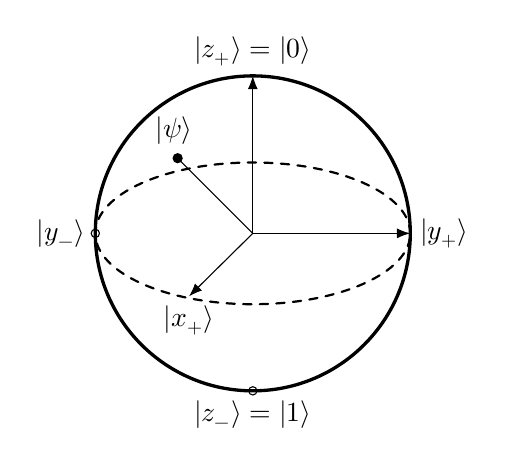
\begin{tikzpicture}[line cap=round, line join=round]
					\draw[very thick] (0,0) circle (2cm);
					\draw[thick, rotate around={0.:(0.,0.)}, dash pattern=on 3pt off 3pt] (0,0) ellipse (2cm and 0.9cm);
					\draw[-Circle] (0,0) -- (-1,1) node[above]{$\ket{\psi}$};
			
					\draw[-Latex] (0,0) -- (0,2) node[above]{$\ket{z_+}=\ket{0}$};
					\draw[-Latex] (0,0) -- (-0.81,-0.8) node[below]{$\ket{x_+}$};
					\draw[-Latex] (0,0) -- (2,0) node[right]{$\ket{y_+}$};
			
					\draw (0,-2) circle (1.5pt) node[below] {$\ket{z_-}=\ket{1}$};
					\draw (-2,0) circle (1.5pt) node[left] {$\ket{y_-}$};
				\end{tikzpicture}
				\caption{Bloch sphere with pure quantum state $\ket{\psi}=c_1\ket{0}+c_2\ket{1}$.}
			\end{figure}
			\column{0.6\textwidth}
			\begin{table}
				\caption{Physical encodings or logical qubit.}
				\begin{tabular}{lcc}
					\toprule
					& \multicolumn{2}{c}{Basis elements} \\
					\cmidrule(lr){2-3}
					&  $\ket{0}$ & $\ket{1}$ \\
					\midrule
					Polarization & Horizontal & Vertical \\
					Photon number & Vacuum & Photon \\
					Time binning & Early & Late \\
					Phase binning & \SI{0}{\degree} & \SI{180}{\degree} \\
					\bottomrule
				\end{tabular}
			\end{table}
		\end{columns}
	\end{frame}
	
	\begin{frame}{Quantum transmission in qubit-based QKD}
		\begin{table}
			\caption{Possible quantum transmission sequence for BB84.}
			\begin{tabular}{lcccccc}
				\toprule
				& \multirow{2}{*}{Step} & \multicolumn{5}{c}{Transmission iteration} \\
				\cmidrule(lr){3-7}
				& & 1 & 2 & 3 & 4 & 5 \\ 
				\midrule
				\multirow{3}{*}{Alice} & Symbol & \num{0} & \num{1} & \num{1} & \num{0} & \num{0} \\
				& Encoding basis & $Z$ & $X$ & $X$ & $Z$ & $X$ \\
				& Prepared state & $\ket{z_+}$ & $\ket{x_-}$ & $\ket{x_-}$ & $\ket{z_+}$ & $\ket{x_+}$ \\
				\cmidrule{1-1}
				\multirow{3}{*}{Bob} & Measurement basis & $X$ & $Z$ & $X$ & $Z$ & $Z$ \\
				& Possible outcomes & \num{0},\num{1} & \num{0},\num{1} & \num{1} & \num{0} & \num{0},\num{1} \\
				& Sifted outcomes & - & - & \num{1} & \num{0} & - \\
				\bottomrule
			\end{tabular}
		\end{table}
	\end{frame}
	
	\begin{frame}{Squeezed-coherent-encoding QKD}
		\begin{figure}
			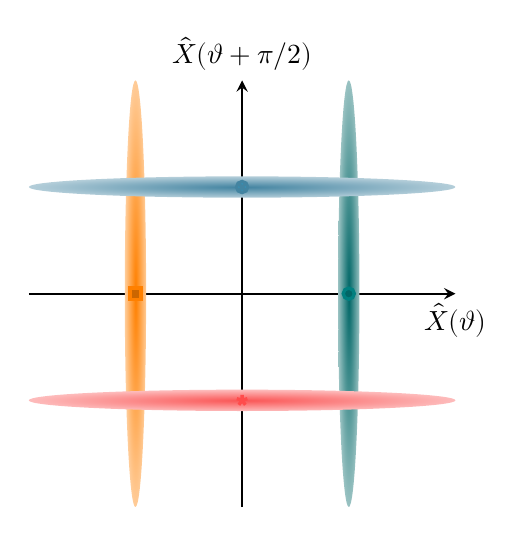
\begin{tikzpicture}
				\begin{axis}[
					height=7cm,
					width=\linewidth,
					axis lines=center,
					axis line style=thick,
					axis equal image,
					xlabel={$\hat{X}(\vartheta)$},
					ylabel={$\hat{X}(\vartheta+\pi/2)$},
					ticks=none,
					xmin=-2,
					xmax=+2,
					ymin=-2,
					ymax=+2,
					axis line style={thick},
					x label style={
						at={(axis description cs:1,0.5)},
						anchor=north,
					},
					y label style={
						at={(axis description cs:0.5,1)},
						anchor=south,
					},
					cycle list name=exotic,
						legend style={
							at={(axis cs: 4,0)},
							anchor=east,
							inner sep=5,
							outer sep=10,
						},
					legend cell align={left},
				]
					\addplot+[very thick] coordinates {(1,0)};
					\addplot+[very thick] coordinates {(-1,0)};
					\addplot+[very thick] coordinates {(0,1)};
					\addplot+[very thick] coordinates {(0,-1)};
		
					\shadedraw[inner color=exotic green, outer color=exotic green!40, draw=none] (axis cs:1,0) ellipse (0.1 and 2);
					\shadedraw[inner color=exotic orange, outer color=exotic orange!40, draw=none] (axis cs:-1,0) ellipse (0.1 and 2);
					\shadedraw[inner color=exotic blue, outer color=exotic blue!40, draw=none] (axis cs:0,1) ellipse (2 and 0.1);
					\shadedraw[inner color=exotic red, outer color=exotic red!40, draw=none] (axis cs:0,-1) ellipse (2 and 0.1);
				\end{axis}
			\end{tikzpicture}
			\caption{Phase space diagram of squeezed-coherent states emulating BB84.}
		\end{figure}
	\end{frame}
	
	\begin{frame}{Coherent-encoding boson-based QKD}
		\begin{figure}
			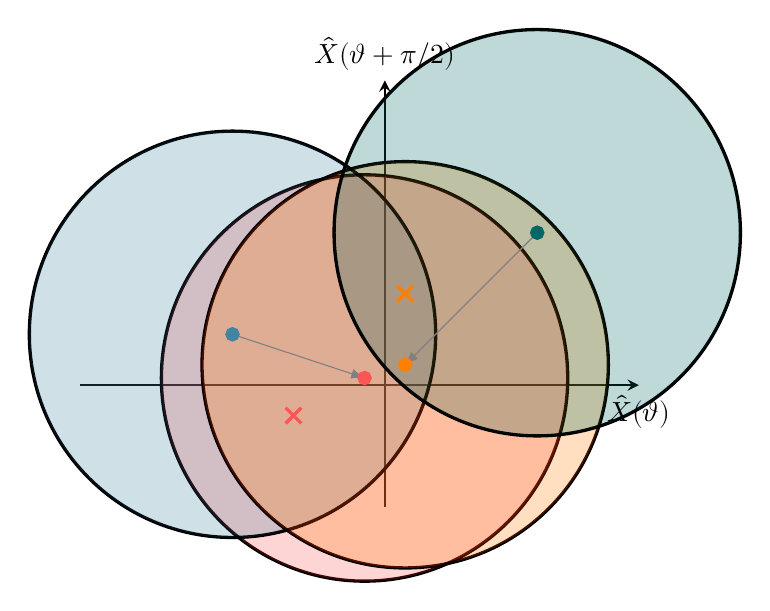
\begin{tikzpicture}[
				var/.style={draw, very thick, fill opacity=0.25, circle, minimum width=45mm},
			]
				\begin{axis}[
					height=7cm,
					width=\linewidth,
					clip=false,
					axis lines=center,
					axis equal image,
					axis line style=thick,
					xlabel={$\hat{X}(\vartheta)$},
					ylabel={$\hat{X}(\vartheta+\pi/2)$},
					ticks=none,
					xmin=-3,
					xmax=+2.5,
					ymin=-1.2,
					ymax=+3,
					axis line style={thick},
					x label style={
						anchor=north,
					},
					y label style={
						anchor=south,
					},
					legend style={
						at={(axis cs:-0.9,2.8)},
						anchor=east,
						draw=none,
						inner sep=5,
						outer sep=10,
					},
					legend columns=2,
					legend cell align={left},
				]
					\begin{scope}[blend group=soft light]					
						\draw[var, fill=exotic green] (axis cs:1.5,1.5) circle (2);
						\draw[var, fill=exotic orange] (axis cs:0.2,0.2) circle (2);
						\draw[var, fill=exotic blue] (axis cs:-1.5,0.5) circle (2);
						\draw[var, fill=exotic red] (axis cs:-0.2,0.07) circle (2);
					\end{scope}

					\addplot[very thick, mark=*, exotic green] coordinates {(1.5,1.5)};	
					\addplot[very thick, mark=*, exotic blue] coordinates {(-1.5,0.5)};	
					\addplot[very thick, mark=*, exotic orange] coordinates {(0.2,0.2)};
					\addplot[very thick, mark=*, exotic red] coordinates {(-0.2,0.07)};
					\addplot[very thick, mark=x, mark size=4, exotic red] coordinates {(-0.9,-0.3)};
					\addplot[very thick, mark=x, mark size=4, exotic orange] coordinates {(0.2,0.9)};
		
					\draw[-Latex, gray] (axis cs:1.5,1.5) -- (axis cs:0.2,0.2);
					\draw[-Latex, gray] (axis cs:-1.5,0.5) -- (axis cs:-0.2,0.07);
				\end{axis}
			\end{tikzpicture}
			\caption{Phase space diagram of coherent states including variance and examples for measurement outcomes.}
		\end{figure}
	\end{frame}
	
	\section{Communication engineering}
	
	\begin{frame}{Pulse-shaping}
		
	\end{frame}
	
	\begin{frame}{Upconversion}
		
	\end{frame}
	
	\begin{frame}{Downconversion}
		
	\end{frame}
	
	\section{Problem and proposed solution}
	
	\begin{frame}{Problem statement}
		\begin{columns}[c, onlytextwidth]
			\column{0.4\textwidth}
			\begin{itemize}
			    \item Foo
			    \item Bar
			    \item Baz
			\end{itemize}
			
			\column{0.4\textwidth}
			\begin{figure}
				\caption{Block diagram of our approach.}
			\end{figure}
		\end{columns}
	\end{frame}
	
	\section{Conclusion and outlook}
	
	\begin{frame}
		\begin{center}
			\textbf{Postlude}
			
			How does light interact with matter?
		\end{center}
	\end{frame}
	
	\appendix
	
	\begin{frame}{Classical post-processing pipeline}
		\begin{figure}
	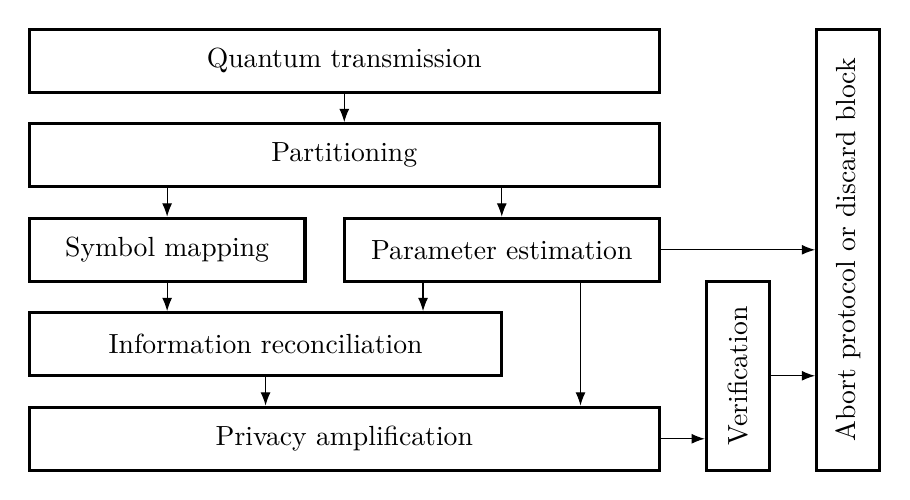
\begin{tikzpicture}[
		block/.style={draw, very thick, minimum height=8mm},
	]
		\node[block, minimum width=8cm] (qt) at (0,0) {Quantum transmission};
		\node[block, minimum width=8cm] (pt) at (0,-1.2) {Partitioning};
		
		\node[block, minimum width=3.5cm] (sm) at (-2.25,-2.4) {Symbol mapping};
		\node[block, minimum width=4cm] (pe) at (2,-2.4) {Parameter estimation};
		\node[block, minimum width=6cm] (ir) at (-1,-3.6) {Information reconciliation};
		\node[block, minimum width=8cm] (pa) at (0,-4.8) {Privacy amplification};

		\draw[-Latex] (qt) -- (pt);
		\draw[Latex-] (sm.north) -- (sm.north|-pt.south);
		\draw[Latex-] (pe.north) -- (pe.north|-pt.south);
		\draw[-Latex] (sm.south) -- (sm.south|-ir.north);
		\draw[-Latex] (ir.south) -- (ir.south|-pa.north);

		\begin{scope}[transform canvas={xshift=-1cm}]
			\draw[-Latex] (pe.south) -- (pe.south|-ir.north);
		\end{scope}
		\begin{scope}[transform canvas={xshift=1cm}]
			\draw[-Latex] (pe.south) -- (pe.south|-pa.north);
		\end{scope}
		
		\node[block, rotate=90, minimum width=2.4cm] (ver) at (5,-4) {Verification};
		\node[block, rotate=90, minimum width=5.6cm] (abort) at (6.4,-2.4) {Abort protocol or discard block};
		\draw[-Latex] (pe.east) -- (pe.east-|abort.north);
		\draw[-Latex] (pa.east) -- (pa.east-|ver.north);
		\draw[-Latex] (ver.south) -- (ver.south-|abort.north);
	\end{tikzpicture}
		\caption{Block diagram of classical post-processing pipeline.}
		\end{figure}
	\end{frame}
	
	% I am a little theory fanboy
	% I think their general methods are often underappreciated
	% However, to me their research problems are too far away from the experiment and self-centered
	\section{Continuous-mode quantum theory of light}
	
	% Lagrangian from first principles (gauge symmetry, vector field, Lorentz scalar, order of derivatives)
	% Field-theoretic framework (energy-momentum tensor, angular momentum tensor, conservation laws, ...)
	% Covariant Maxwell equations follow directly
	\begin{frame}{Maxwell Lagrangian and equations}
		The Lagrangian density for the Maxwell field $A^\mu(t,\vb{x})$
		\begin{equation}
			\mathcal{L}
			=
			-
			\frac{1}{4}
			F_{\mu\nu}
			F^{\mu\nu}
			+
			A_\mu j^\mu
			,
		\end{equation}
		wherein
		\begin{align}
			F_{\mu\nu}
			&=
			\partial_\mu
			A_\nu
			-
			\partial_\nu
			A_\mu
			&
			\tilde{F}^{\mu\nu}
			&=
			\frac{1}{2}
			\varepsilon^{\mu\nu\rho\sigma}
			F_{\rho\sigma}
		\end{align}
		and employing variational calusu and the Bianchi identity lead us to the covariant formulation of the Maxwell equations
		\begin{align}
			\partial_\mu
			\tilde{F}^{\mu\nu}
			&=
			0
			&
			\partial_\mu
			F^{\mu\nu}
			&=
			j^\mu
			.
		\end{align}
	\end{frame}

	% interpretation of temporal and Coulomb gauge
	% alternative to Lorenz gauge, we choose a gauge transform to remove non-transverse DOFs
	% expectation value of the Maxwell field operator w.r.t. a coherent state
	% Coulomb gauge in momentum space requires polarization vectors to be orthogonal to momentum vector
	\begin{frame}{Transverse plane-wave expansion}
		\begin{columns}[c, onlytextwidth]
			\column{0.5\textwidth}
			Temporal and Lorenz gauge
			\begin{equation}
				A_0
				=
				0
				\quad
				\text{and}
				\quad
				\partial_i
				A^i
				=
				0
			\end{equation}
			the field becomes transverse and the equation of motion reduces to a relativistic wave equation
			\begin{equation}
				\partial_t^2
				\vb{A}
				=
				\laplace
				\vb{A}
			\end{equation}
			\begin{equation}
				\vb{A}(t,\vb{x})
				=
				\int\frac{\dd[4]{p}}{(2\pi)^4}
				\vb{A}(p_0,\vb{p})
				e^{-ip_0t+i\vb{p}\vdot\vb{x}}
			\end{equation}
			
			\column{0.5\textwidth}
			\begin{equation}
				p_0
				=
				\omega(\vb{p})
				=
				\norm{\vb{p}}
			\end{equation}
			\begin{equation}
				\vb{A}(t,\vb{x})
				=
				\int\frac{\dd[3]{p}}{(2\pi)^3\sqrt{2\omega(\vb{p})}}
				\vb{A}\!\left(\omega(\vb{p}),\vb{p}\right)
				+
				\text{c.c.}
			\end{equation}
			\begin{equation}
				\vb{A}\!\left(\omega(\vb{p}),\vb{p}\right)
				=
				\sum_{\lambda=1,2}
				a_\lambda(\vb{p})
				\hat{a}_\lambda(\vb{p})
				\vu{e}_\lambda(\vb{p})
			\end{equation}
		\end{columns}
	\end{frame}
	


	\begin{frame}{Canonical quantization in the Coulomb gauge}
		\begin{align}
			\vu{A}^{(-)}(t,\vb{x})
			&=
			\sum_{\lambda=1,2}
			\int\frac{\dd[3]{p}}{(2\pi)^3\sqrt{2\omega(\vb{p})}}
			\hat{a}_\lambda(\vb{p})
			\vu{e}_\lambda(\vb{p})
			e^{-i\omega(\vb{p})t+i\vb{p}\vdot\vb{x}}
			\\
			\vu{E}^{(-)}(t,\vb{x})
			&=
			-i
			\sum_{\lambda=1,2}
			\int\frac{\dd[3]{p}}{(2\pi)^3\sqrt{2\omega(\vb{p})}}
			\omega(\vb{p})
			\hat{a}_\lambda(\vb{p})
			\vu{e}_\lambda(\vb{p})
			e^{-i\omega(\vb{p})t+i\vb{p}\vdot\vb{x}}
		\end{align}
		\begin{align}
			\comm{\hat{A}_i(t,\vb{x})}{\hat{E}_j(t,\vb{y})}
			&=
			-i\delta_{\perp ij}^{(3)}(\vb{x}-\vb{y})
			\\
			\comm{\hat{A}_i(t,\vb{x})}{\hat{A}_j(t,\vb{y})}
			&=
			\comm{\hat{E}_i(t,\vb{x})}{\hat{E}_j(t,\vb{y})}
			=
			0
		\end{align}
		\begin{align}
			\hat{H}
			&=
			\sum_{\lambda=1,2}
			\int\frac{\dd[3]{p}}{(2\pi)^3}
			\omega(\vb{p})
			\hat{a}_\lambda^\dagger(\vb{p})
			\hat{a}_\lambda(\vb{p})
			&
			\vu{P}
			&=
			\sum_{\lambda=1,2}
			\int\frac{\dd[3]{p}}{(2\pi)^3}
			\vb{p}
			\hat{a}_\lambda^\dagger(\vb{p})
			\hat{a}_\lambda(\vb{p})
		\end{align}
	\end{frame}
	
	\begin{frame}{Number state}
		\begin{equation}
			\begin{split}
				\ket{n_f}
				=
				\frac{1}{\sqrt{n!}}
				\hat{A}^{(+)}[f]^n
				\ket{0}
				&=
				\frac{1}{\sqrt{n!}}
				\left(
					\int\dd[4]{x}
					f(t,\vb{x})
					\hat{A}^{(+)}(t,\vb{x})
				\right)^n
				\ket{0}
				\\
				&=
				\frac{1}{\sqrt{n!}}
				\left(
					\int\frac{\dd[3]{p}}{(2\pi)^3\sqrt{2\omega(\vb{p})}}
					f\!\left(\omega(\vb{p}),\vb{p}\right)
					\hat{A}^{(+)}(t,\vb{x})
					\hat{a}^\dagger(\vb{p})
				\right)^n
				\ket{0}
			\end{split}
		\end{equation}
		\begin{equation}
			\braket{1_f}{1_f}
			=
			\int\frac{\dd[3]{p}}{(2\pi)^3}
			\abs*{\frac{f\!\left(\omega(\vb{p}),\vb{p}\right)}{\sqrt{2\omega(\vb{p})}}}^2
			=
			1
		\end{equation}
		\begin{equation}
			\bra{n_f}
			\hat{H}
			\ket{n_f}
			=
			n
			\int\frac{\dd[3]{p}}{(2\pi)^3}
			\omega(\vb{p})
			\abs*{\frac{f\!\left(\omega(\vb{p}),\vb{p}\right)}{\sqrt{2\omega(\vb{p})}}}^2
		\end{equation}
	\end{frame}

	\begin{frame}{Coherent state}
		\begin{equation}
			\hat{\alpha}
			=
			\hat{D}\left[\alpha\right]
			\ket{0}
		\end{equation}
		\begin{equation}
			\begin{split}
				\hat{D}\left[\alpha\right]
				&=
				\exp\biggl\{
					\hat{A}^{(+)}[\alpha]
					-
					\hat{A}^{(-)}[\alpha^*]
				\biggr\}
				\\
				&=
				\exp\left\{
					\int\frac{\dd[3]{p}}{(2\pi)^3\sqrt{2\omega(\vb{p})}}
					\left[
						\alpha(\vb{p})
						\hat{a}^\dagger(\vb{p})
						-
						\alpha(\vb{p})^*
						\hat{a}(\vb{p})
					\right]
				\right\}
			\end{split}
		\end{equation}
	\end{frame}

\end{document}